% Created 2023-10-23 Mon 23:00
% Intended LaTeX compiler: pdflatex
\documentclass[presentation,smaller]{beamer}
\usepackage[utf8]{inputenc}
\usepackage[T1]{fontenc}
\usepackage{graphicx}
\usepackage{longtable}
\usepackage{wrapfig}
\usepackage{rotating}
\usepackage[normalem]{ulem}
\usepackage{amsmath}
\usepackage{amssymb}
\usepackage{capt-of}
\usepackage{hyperref}
\usetheme{MIS}
\author{vopuu}
\date{\today}
\title{}
\begin{document}


\section*{SHALLOW PART}
\label{sec:org8373cf6}

\begin{frame}[label={sec:orgd2983e0}]{Challenges of Physics-Based Approaches}
\begin{itemize}
\item \alert{\alert{Computational Intensity}}: Demanding molecular dynamics simulations.
\item \alert{\alert{Incomplete Modeling}}: Often neglects complex environmental interactions.
\end{itemize}
\end{frame}

\begin{frame}[label={sec:org45a2c8d}]{Nature's Blueprint}
\begin{itemize}
\item \alert{\alert{Evolutionary optimization}}: Natural proteins are optimized to the physical
diffusion limits.
\item \alert{\alert{Homology Modeling}}: Borrowing structures from evolutionarily related proteins.
\item \alert{\alert{Evolutionary Couplings}}: Pinpointing residues crucial for function.
\item \alert{\alert{Advantages}}:
\begin{itemize}
\item Sidestep computational hurdles.
\item Tap into nature's tried-and-tested designs.
\end{itemize}
\end{itemize}
\end{frame}

\section*{MSA now}
\label{sec:org8cd3381}

\begin{frame}[label={sec:orgdabadae}]{How to extract these fined-tuend proteins, and what to do?}
\begin{center}
\Large \textbf{Given a target natural function, search for natural counterparts}
\end{center}
\end{frame}

\begin{frame}[label={sec:org91b69ee}]{Typical approach}
\begin{center}
\Large
\begin{enumerate}
\item Search natural counterparts for a targeted function.
\item Extract statistical signature from the collection of natural sequences.
\item Use the statistical signature to sample novel sequences.
\end{enumerate}
\end{center}
\end{frame}

\begin{frame}[label={sec:org9d42c83}]{Multiple Sequence Alignments (MSAs) - the data}
\begin{itemize}
\item Definition: Aligning multiple sequences to identify regions of similarity.
\item Importance in bioinformatics:
\begin{itemize}
\item Studying phylogenetics and evolutionary processes.
\item Identifying protein domains.
\end{itemize}
\end{itemize}

\begin{center}
\begin{center}
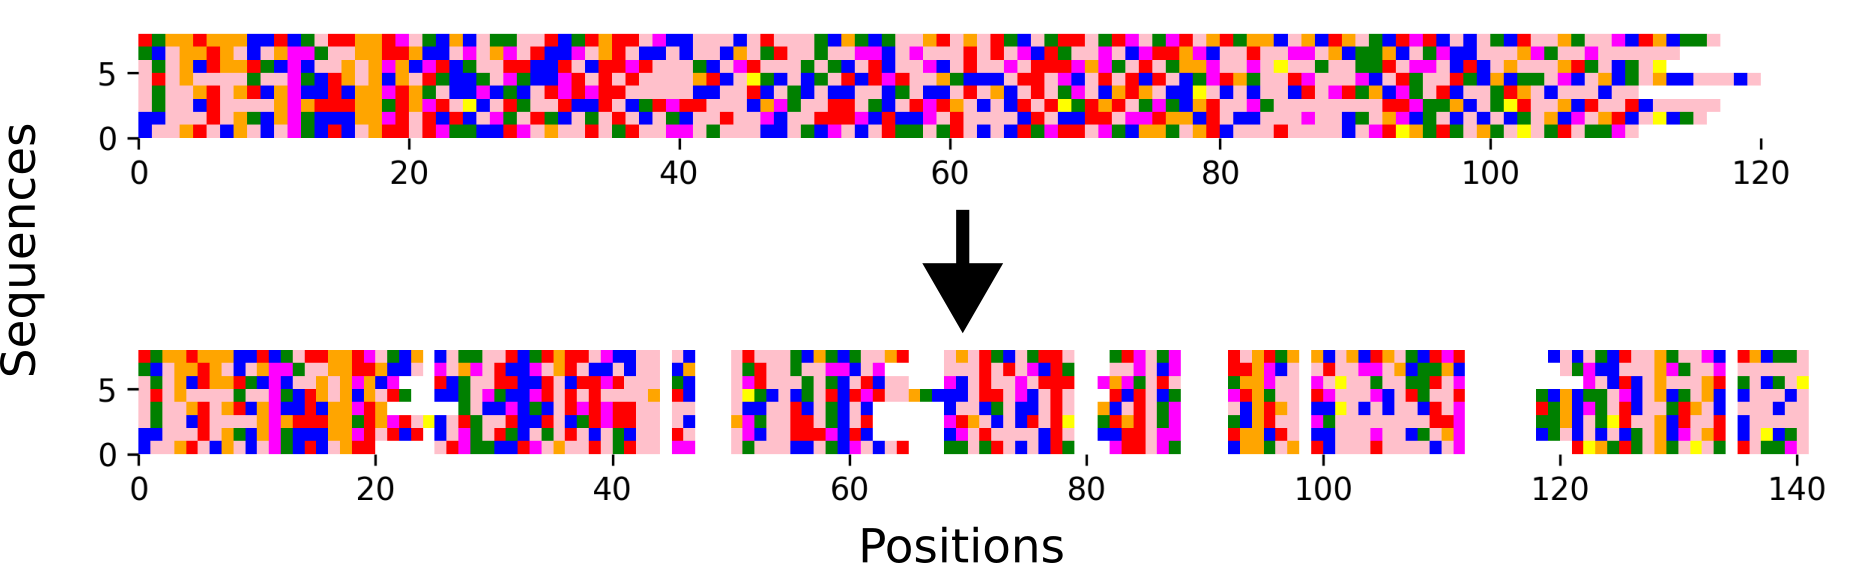
\includegraphics[width=.9\linewidth]{./img/msa.png}
\end{center}
\end{center}
\end{frame}

\begin{frame}[label={sec:org84684a9}]{Multiple Sequence Alignments (MSAs) - the data}
\begin{columns}
\begin{column}{0.6\columnwidth}
\begin{itemize}
\item Information extraction from MSAs:
\begin{itemize}
\item Phylogenetic trees: Tracing evolutionary pathways.
\item Functional domains \& conserved motifs: Identifying patterns.
\item Critical residues for protein function or stability.
\end{itemize}
\item Popular tools \& databases for MSAs:
\begin{itemize}
\item Clustal: Widely used for sequence alignment.
\item Pfam: Database of protein families based on MSAs.
\item Uniprot: Comprehensive protein database.
\end{itemize}
\end{itemize}
\end{column}

\begin{column}{0.4\columnwidth}
\begin{center}
\begin{center}
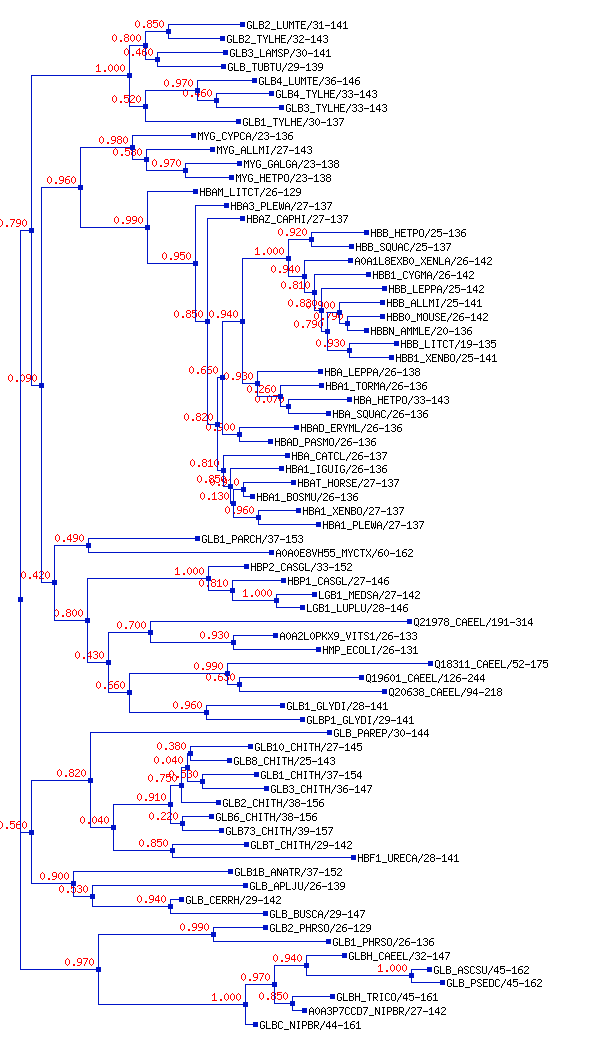
\includegraphics[width=.9\linewidth]{./img/pfam.png}
\end{center}
\end{center}
\end{column}
\end{columns}
\end{frame}

\begin{frame}[label={sec:orgc02bc99}]{Encoding MSAs for numerical use}
\begin{itemize}
\item MSA is discrete qualitative data type
\end{itemize}

\begin{center}
\textbf{How to use them?}
\end{center}

\begin{block}{Encoding}
\begin{itemize}
\item One-hot:
\end{itemize}
\begin{equation*}
\begin{split}
A \rightarrow \begin{pmatrix} 1\\ 0\\ \dots \\ 0\\ 0 \end{pmatrix},
C \rightarrow \begin{pmatrix} 0\\ 1\\ \dots \\ 0\\ 0 \end{pmatrix},
\dots
Y \rightarrow \begin{pmatrix} 0\\ 0\\ \dots \\ 1\\ 0 \end{pmatrix},
W \rightarrow \begin{pmatrix} 0\\ 0\\ \dots \\ 0\\ 1 \end{pmatrix}.
\end{split}
\end{equation*}
\begin{itemize}
\item Random projection
\item Deep learning embeddings
\end{itemize}
\end{block}
\end{frame}

\begin{frame}[label={sec:org197a352}]{Let's look at the distribution of sequences}
\begin{center}
\Large \textbf{Since we have numerical data, we can also use dimensionality reduction techniques}
\end{center}
\end{frame}

\section*{Visualization}
\label{sec:org7c93b1f}
\begin{frame}[label={sec:orgfde59d5}]{Singular Value Decomposition (SVD) for Protein Data}
\begin{columns}
\begin{column}{0.6\columnwidth}
\begin{itemize}
\item \alert{\alert{Application}}: Extracting meaningful patterns from vast protein datasets.
\item \alert{\alert{Dimensionality Reduction}}: Simplifies complex data, retaining essential information.
\item \alert{\alert{Pattern Recognition}}: Reveals underlying structures and relationships in protein data.
\end{itemize}
\end{column}

\begin{column}{0.4\columnwidth}
\begin{center}
\begin{center}
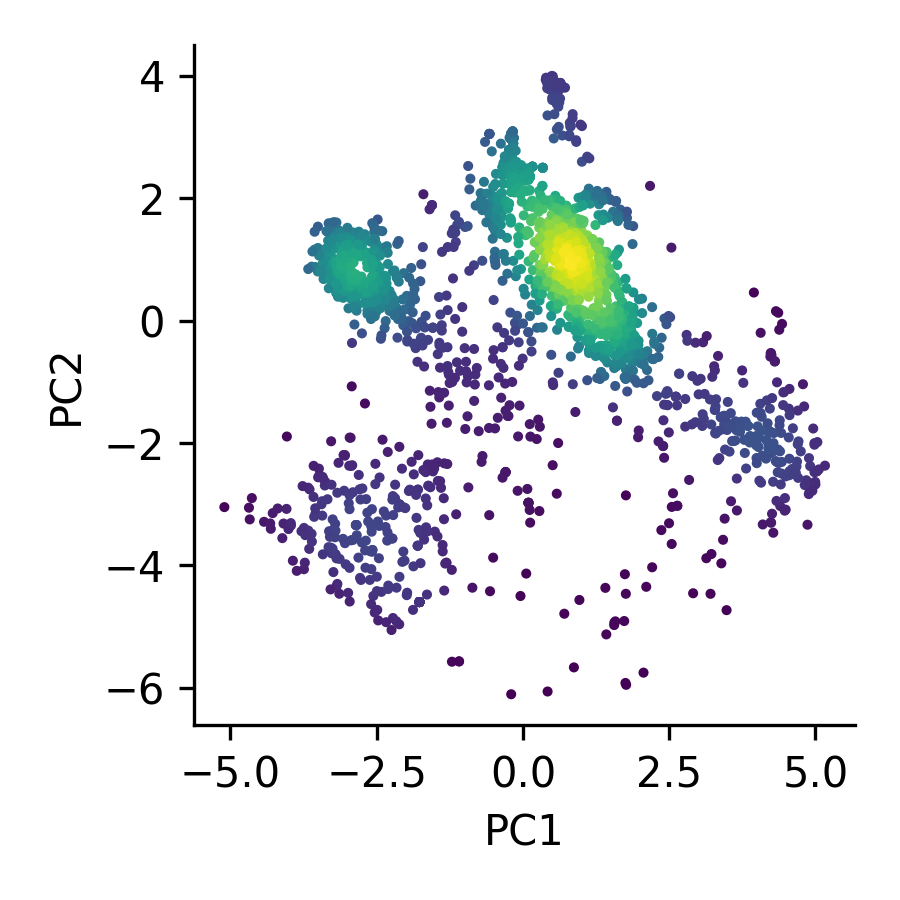
\includegraphics[width=.9\linewidth]{./img/svd_pfam.png}
\end{center}
\end{center}
\end{column}
\end{columns}
\end{frame}

\begin{frame}[label={sec:orgef59855}]{Mathematics behind SVD}
\begin{block}{Introduction}
\begin{itemize}
\item Fundamental technique in linear algebra.
\item Decomposes a matrix into three other matrices.
\item Widely used in data compression, noise reduction, and more.
\end{itemize}
\end{block}

\begin{block}{Mathematical Representation}
\begin{itemize}
\item Given a matrix \(MSA\):
\[ MSA = U \Sigma V^T \]
Where:
\begin{itemize}
\item \(U\) - Left singular vectors (orthogonal matrix).
\item \(\Sigma\) - Diagonal matrix of singular values.
\item \(V^T\) - Transpose of right singular vectors (orthogonal matrix).
\end{itemize}
\end{itemize}
\end{block}
\end{frame}

\begin{frame}[label={sec:org970da9f}]{What's in those singular vectors ?}
\alert{*}
\begin{itemize}
\item The right singular vectors correspond to compositional motifs (in terms of
sequences).
\end{itemize}

\begin{center}
\begin{center}
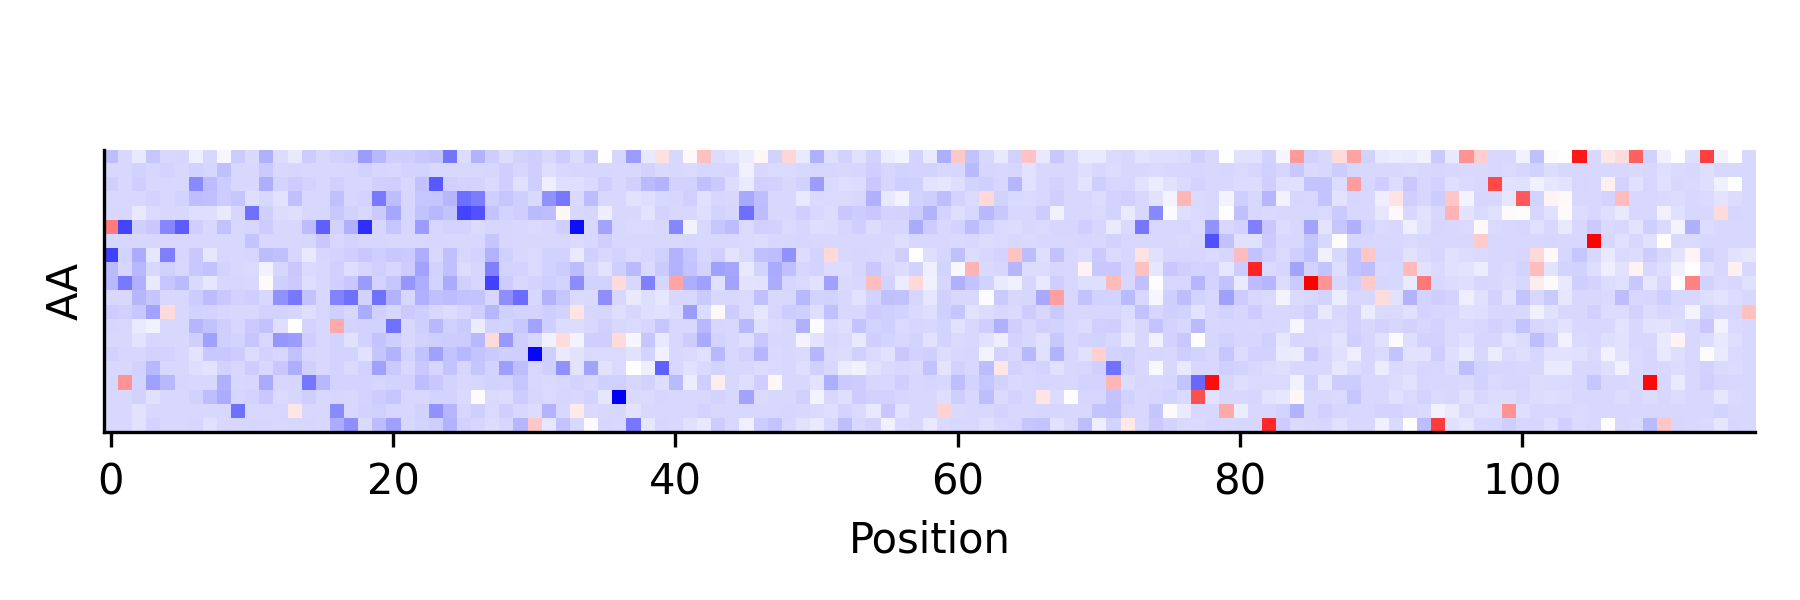
\includegraphics[width=.9\linewidth]{./img/svd_pfam_vec_1.png}
\end{center}
\end{center}
\end{frame}

\begin{frame}[label={sec:org9d0e309}]{Sample compositional motifs}
\begin{center}
\Large \textbf{Sample the compositional motifs observed in the MSA to form novel sequences}
\end{center}
\end{frame}

\begin{frame}[label={sec:orge56b6f3}]{Sequence Generation using SVD}
\begin{itemize}
\item Concept of reverse mapping: Generating functional sequences from
reduced-dimensional data.
\end{itemize}

\begin{center}
\begin{center}
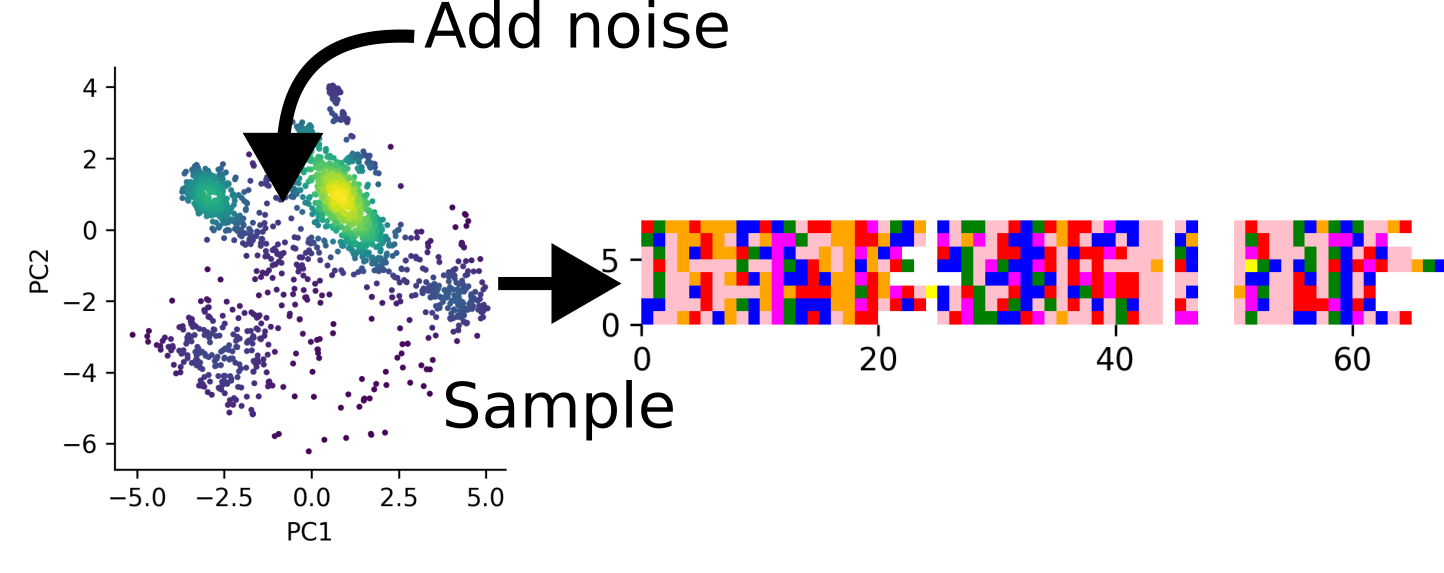
\includegraphics[width=.9\linewidth]{./img/svd_design.png}
\end{center}
\end{center}

Introduce a Gaussian blank noise to sample the PCs:

\begin{equation*}
\begin{split}
\tilde{U} =  U + \mathcal{N}(0, 1)\\
\hat{MSA} = \tilde{U} \Sigma V^T
\end{split}
\end{equation*}
\end{frame}

\section*{DCA}
\label{sec:orgaae71fa}
\begin{frame}[label={sec:orgb0f234e}]{A pairwise model borrowed from statistical physics}
\begin{center}
\Large \textbf{Direct coupling analysis}
\end{center}

F. Morcos \emph{et al}, PNAS 2011
\end{frame}

\begin{frame}[label={sec:orgb55a935}]{Markov Random Field for Protein Analysis}
\begin{itemize}
\item Parametrize a probability distribution describing the distribution of sequences.
\item Decompose the complex distribution of sequences into a pairwise potential ---
the Potts model.
\end{itemize}

\begin{center}
\begin{center}
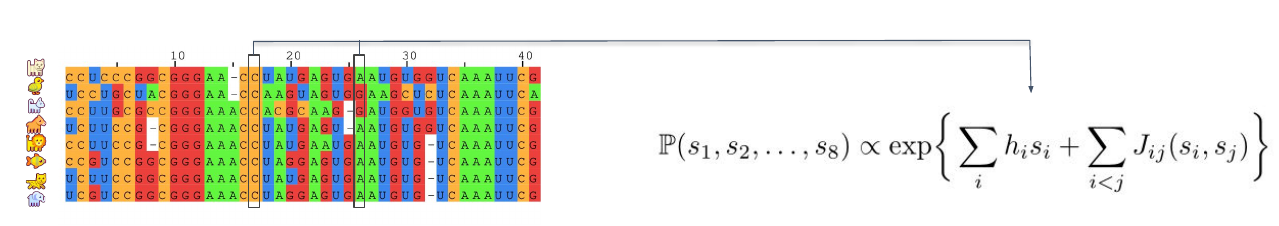
\includegraphics[width=.9\linewidth]{./img/dca_image.png}
\end{center}
\end{center}
\end{frame}

\begin{frame}[label={sec:org17a6da8}]{Mathematics behind Random Markov Fields}
\begin{block}{MSA probabilistic model [Morcos \emph{et al}, PNAS, 2011]}
\begin{itemize}
\item Probability associated to a Sequence given a MSA:
\end{itemize}
\begin{equation*}
P_{\mathcal{H}}(S) \propto \text{exp}\{-\beta \times \mathcal{H}(S)\}
\end{equation*}
\begin{itemize}
\item Energy of a sequence (Potts models):
\end{itemize}
\begin{equation*}
\mathcal{H}(S) = \displaystyle\sum_{i} h_i(S_i) + \displaystyle\sum_{i<j} J_{ij}(S_i,S_j)
\end{equation*}
\begin{itemize}
\item Energy parameters:
\begin{itemize}
\item \(\mathcal{H} = \{h_i; J_{ij}\}\) (lookup table)
\item Parameter space: \(5 \times L + 5^2 \times \frac{L \times (L - 1)}{2} = 464165\)
\end{itemize}
\end{itemize}
\end{block}
\end{frame}

\begin{frame}[label={sec:org68aa3de}]{Initial applications of DCA}
Contact predictions based on coupling terms \(J_{ij}\):
\begin{equation*}
F_{ij} &= \sqrt{\sum J_{ij}(A,B)^2} \;\;\; \rightarrow \;\;\; F^{APC}_{ij} &= F_{ij} - \frac{F_{i.}F_{.j}}{F_{..}}
\end{equation*}
\end{frame}

\begin{frame}[label={sec:org5d7f7b8}]{DCA learning technique}
\begin{block}{Turn into an optimization procedure}
\begin{itemize}
\item Fit low-order statistics such as \(f_i\) and \(f_{ij}\): Find \(\mathcal{H}\) such that:
\end{itemize}
\begin{equation*}
\hat{f}_{i}(A) = f_i(A)\;\;\; ; \;\;\; \hat{f}_{ij}(A,B) = f_{ij}(A,B)
\end{equation*}
\end{block}

\begin{block}{Boltzmann machine learning [Figliuzzi \emph{et al}, Mol. Biol Ev., 2018; Cuturello \emph{et al}, RNA, 2020]}
Initialize with a guess for \(\mathcal{H}\) (could be zeros)
\begin{enumerate}
\item Generate a sample given \(\mathcal{H}\) (MCMC) and compute \(\hat{f}_{i},
  \hat{f}_{ij}\)
\item \(\mathcal{H}\) parameters are updated following the \alert{log-likelihood}
\end{enumerate}
\begin{equation*}
h_i(A) \leftarrow h_i(A) + \eta (\hat{f}_{i}(A) - f_i(A))
\end{equation*}
\end{block}
\end{frame}

\begin{frame}[label={sec:org3696fe2}]{Sequence Generation using Random Markov Field}
\begin{itemize}
\item Sampling sequences: sampling new protein variants.
\item Ensuring biological relevance: Satisfying coevolutionary constraints.
\end{itemize}

Perform mutations:
\begin{center}
\begin{center}
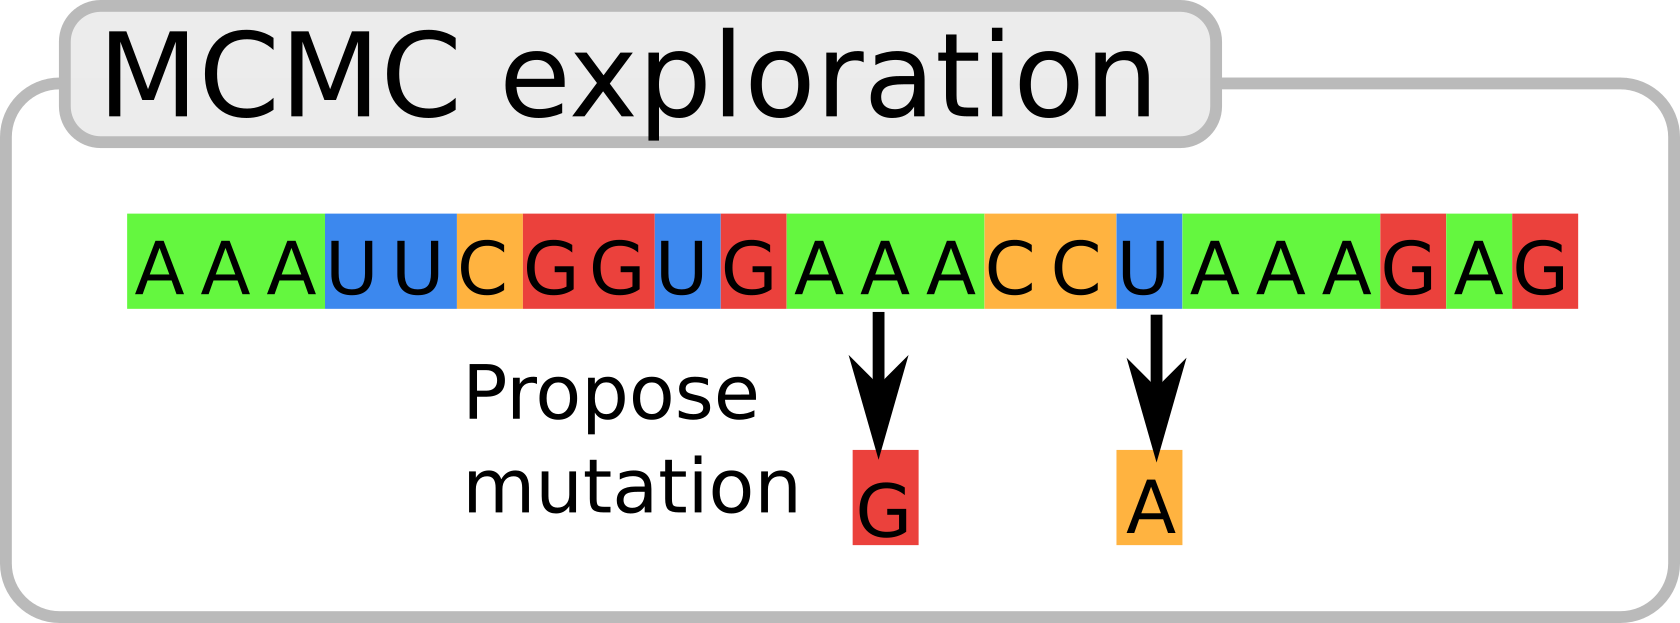
\includegraphics[scale=0.3]{./img/mcmc_seq.png}
\end{center}
\end{center}

Select using the parametrized distribution:
\begin{equation*}
P_{\mathcal{H}}(S) \propto \text{exp}\{-\beta \times \mathcal{H}(S)\}
\end{equation*}
\end{frame}
\end{document}